\documentclass[paper=a4,11pt,titlepage,twoside=true,headings=normal,numbers=noenddot,captions=tableabove,listof=totoc,index=totoc,bibliography=totoc]{scrreprt}
%\usepackage{amsmath} % abgesetzte Formeln zentriert in der Zeile
%\usepackage[fleqn,intlimits]{amsmath} % [fleqn] abgesetzte Formeln mit festem Abstand zum linken Rand
\usepackage[reqno,intlimits]{amsmath} % [reqno] um die gleichungsnummerierung rechts zu haben
% intlimits: Grenzen für Integrale unterhalb und oberhalb des Zeichens
\usepackage{amssymb}
\usepackage{array}
%\usepackage[ngerman]{babel}
%\usepackage[ngerman]{varioref}
\usepackage[english]{babel}
\usepackage[english]{varioref}
\usepackage[T1]{fontenc} 
\usepackage[utf8]{inputenc}
%---------------------------
\usepackage{booktabs}
\usepackage{calc}
\usepackage{cancel}
\usepackage[labelfont={footnotesize,sf,bf},textfont={footnotesize,sf}]{caption} %Format (Textgröße, Textform) für Bildtext 
%normalsize
%scriptsize
% sc --> smallcaps
% bf --> bold face
% sf --> sans serif
%\usepackage{cite} %inkompatibel mit biblatex
\usepackage[table]{xcolor}
%\usepackage{colortbl}
\usepackage[right]{eurosym}
%\usepackage{caption2} %nicht zusammen mit sidecap
%\usepackage{exscale}
\usepackage{ellipsis}
\usepackage{graphicx}
\usepackage{float}
%\usepackage{floatflt}
%----------------------------------------
\usepackage{gensymb} %-----------
%\usepackage{helvet}
\usepackage{csquotes}
\usepackage{listings}
\usepackage{longtable}
\usepackage{lastpage}  %----------
\usepackage{lscape}
\usepackage{lmodern}  %-- Silbentrennung
%\usepackage{mathpazo} % andere mathematische Symbol
\usepackage{makeidx}
%\usepackage{minitoc}
\usepackage{multirow}
\usepackage{multicol}
%\usepackage[intoc]{nomencl}   % zwei Spalten beim Formelzeichenverzeichnis
%\usepackage[german,intoc]{nomentbl} %vier Spalten bei Formelzeichenverzeichnis
\usepackage[english,intoc]{nomentbl} %vier Spalten bei Formelzeichenverzeichnis
\usepackage{nicefrac} %----
%\usepackage{picins} %----------
\usepackage{paralist} %--------
\usepackage{parallel}  %----------
\usepackage{pdfpages} %-------
% Define user colors using the RGB model
%\usepackage{colortbl}
%\definecolor{dunkelgrau}{rgb}{0.8,0.8,0.8}
%\definecolor{hellgrau}{rgb}{0.95,0.95,0.95}
%\usepackage{pgfplots}
\usepackage[figuresright]{rotating} 
\usepackage{scrlayer-scrpage}
%\usepackage[innercaption]{sidecap} %Beschriftung neben Bild, Tabelle, Mittelbach S333 %----------
%\usepackage{sistyle}
%\usepackage[locale=DE]{siunitx} %nicht zusammen mit sistyle %---------
\usepackage[locale=DE,per-mode=symbol,parse-numbers=false]{siunitx} %nicht zusammen mit sistyle %---------
\usepackage[font={scriptsize,sl},captionskip=3pt]{subfig} % für die Unterbilder %---------
\usepackage{shortvrb}
\usepackage{tablefootnote}
\usepackage{tabularx}
\usepackage{tabulary}
\usepackage{textcomp}
\usepackage{tocbasic}
%\usepackage{tikz}
\usepackage{times} 
\usepackage{units} %----------
\usepackage{url}
\usepackage{wrapfig} %----------
\usepackage{xr-hyper}
\usepackage{arydshln} %für \hdashline[5pt/2pt] % muss am Ende stehen, sonst gibt es Probleme mit xcolor
\usepackage{hyperref} % muss am Schluss stehen
\hypersetup{linkcolor={0 1 1}, linkbordercolor={1 1 1}, citebordercolor={1 1 1}} % setzt Linkboxen auf Farbe "`weiß"'
%\usepackage{bm}
%\usepackage[toc,symbols]{glossaries} %---------- muss nach hyperref stehen
\usepackage[nonumberlist, acronym, toc, section]{glossaries} % muss nach hypersetup stehen
%----------------
%\usepackage{romannum} % Seitenzahlen in römischen Ziffern
%\usepackage{adjustbox}
\usepackage{scrhack}
\usepackage[style=phys, citestyle=numeric, backend=biber]{biblatex}
\usepackage[useregional]{datetime2}
\usepackage{cleveref} % löscht labels!!!!!!!!!! <--- warum? habs trotzdem eingefügt weil es die referencen nice macht ohne newcommands dafür zu brauchen. außerdem steht intellisense drauf ;)
%-------------------------
 %\renewcommand{\captionlabelfont}{\sffamily} %für "Abbildung" und "Tabelle"
 %\renewcommand{\captionfont}{\sffamily\small} %für den Text der Bildunterschriften
%  \renewcommand{\captionlabelfont}{\sffamily} 
%  \renewcommand{\captionfont}{\sffamily} %\renewcommand{\normalfont}{\sffamily} %für die Überschriften
% Fettdruck der Bezeichnung Abbildung, Tabelle
%\renewcommand{\captionlabelfont}{\bfseries}
%---------------------------------------------
%------------------ Schrifttyp in der Kopf- und Fusszeilen
\setkomafont{pageheadfoot}{\footnotesize\sffamily}
%---------------------------------------------------
%Ändern der Abbildung- und Tabellenbezeichnung (Niedermair S.157)
%_____________________________________________
\addto\captionsngerman{\renewcommand\figurename{Abb.}}
\addto\captionsngerman{\renewcommand\tablename{Tab.}}
\renewcommand\listfigurename{Abbildungen}
%_______________________________
%Betrag eines Wertes
\newcommand{\abs}[1]{\lvert #1 \rvert} 
%---------------------------------------------
\newcommand{\absatz}[1]{\textbf{\textsc{#1}}} %siehe Mittelbach S. 876ff
%----------------------------
%\newcommand{\absatz}{\par \medskip}
%______________________________
%\newcommand{\anhang}[1]{Anhang \ref{#1}, Seite \pageref{#1}}
\newcommand{\anhang}[1]{Anhang \vref{#1}}
%________________________________
\newcommand{\aufgabe}{\stepcounter{plus} Aufgabe \arabic{plus}}
%______________________________________
%compactitem
\newcommand{\bci}{\begin{compactitem}}
\newcommand{\eci}{\end{compactitem}}
%______________________________________
%
\newcommand{\bi}{\begin{itemize}}
\newcommand{\ei}{\end{itemize}}
%______________________________________
%compactenumerate
\newcommand{\bce}{\begin{compactenum}}
\newcommand{\ece}{\end{compactenum}}
%_____________________________________
%begin equation
\newcommand{\be}{\begin{equation}}
\newcommand{\ee}{\end{equation}}
%_____________________________________
%begin equation ohne Formelnummer
\newcommand{\ben}{\begin{equation*}}
\newcommand{\een}{\end{equation*}}
%_____________________________________
%begin align ohne Formelnummer
\newcommand{\ban}{\begin{align*}}
\newcommand{\ean}{\end{align*}}
%_____________________________________
%begin align
\newcommand{\ba}{\begin{align} }
\newcommand{\ea}{\end{align}}
%_____________________________________
%minpage
\newcommand{\bmp}{\begin{minipage}[t]{.47\linewidth}}
\newcommand{\emp}{\end{minipage}}
%_____________________________
%  dB
\newcommand{\db}{dB}
%  dB(A)
\newcommand{\dba}{ dB(A) }
%  dB(A) für Satzende
\newcommand{\dbap}{ dB(A)}
%_________________________________
\newcommand{\bzw}{bzw.\,}
%_______________________________
\newcommand{\dif}{\mathrm{d}}
%________________________________
% neuer Zähler
\newcounter{plus}
\setcounter{plus}{0}
%______________________________
%Für das Formelverzeichnis _____________________ Formelverzeichis ____
% Befehl umbenennen in fz
\let\fz\nomenclature
% Deutsche Überschrift
\renewcommand{\nomname}{Formelzeichen}
% Punkte zw. Abkürzung und Erklärung
\setlength{\nomlabelwidth}{.20\hsize}
\renewcommand{\nomlabel}[1]{#1 \dotfill}
% Zeilenabstände verkleinern
\setlength{\nomitemsep}{-\parsep}
%_____________________________
\newcommand{\bild}[1]{Abb. \vref{#1}}
\newcommand{\sbild}[1]{siehe Abb. \vref{#1}}
\newcommand{\bilder}[2]{Abb. \vrefrange{#1}{#2}}
\newcommand{\bildseite}[1]{Abb. \vref{#1}} % erzeugt "`Abb. nn auf Seite nn
\newcommand{\tabelle}[1]{Tab. \vref{#1}}
\newcommand{\tabellenseite}[1]{Tab. \vref{#1}} % erzeugt "`Tab. nn auf Seite nn
% für \vref ist usepackage[german]{varioref} einzufügen
%_-------------------------------- Freiraum
\newcommand{\freiraum}[1]{\begin{figure}[H]\vspace{#1\textheight}\end{figure}}
%_____________________________
% Gleichung
\newcommand{\gl}[1]{Gl.\,(\ref{#1})}
\newcommand{\sgl}[1]{siehe Gl.\,(\ref{#1})}
\newcommand{\glbereich}[2]{Gl. \vrefrange[]{#1}{#2}}
%_____________________________
% Grad Celsius
\newcommand{\grad}{\,\degC}
\newcommand{\gradC}{\,\degree}
%______________________________________
% Großbuchstaben als Indizes kleiner schreiben; spezielle im Mathemodus
\newcommand{\klein}[1]{\scriptscriptstyle{#1}}% Fettdruck der Bezeichnung 
%______________________________
%% Kasten
\newcommand{\kasten}{\fbox{\rule{0.0pt}{10pt}{{ } } }}
%______________________________
%\newcommand{\kapitel}[1]{Kapitel \ref{#1}, Seite \pageref{#1}}
\newcommand{\kapitel}[1]{Kapitel \vref{#1}}
%_____________________________
%  LAeq für den äquivalenten Dauerschallpegel
\newcommand{\laeq}{ $L_{Aeq}$ }
%  LAeq für den äquivalenten Dauerschallpegel am Satzende
\newcommand{\laeqp}{ $L_{Aeq}$}
%_________________________________
%   Linie zeichnen
\newcommand{\linie}{\rule{0.5\textwidth}{0.1pt}}
%---------------------- LaTeX
\newcommand{\lt}{\LaTeX\,\,}
%----------------------------
\newcommand{\nl}{\newline}
%__________________________________
%  multicolumn für Tabellen
\newcommand{\mc}{\multicolumn}
%% \mc{1}{c}{Text}
%_________________________________
%    Parallel
\newcommand{\pl}[1]{\ParallelLText{#1}}
\newcommand{\pr}[1]{\ParallelRText{#1}}
\newcommand{\pp}{\ParallelPar}
%------------ rot unterstrichen
\newcommand{\rotunterstrichen}[1]{\textcolor{red}{\underline{\textcolor{black}{#1}}}}
%________________ Realteil
\newcommand{\real}[1]{\text{Re}\left\{#1\right\}}
%________________________________--
\newcommand{\seite}[1]{Seite \pageref{#1}}
\newcommand{\seiten}[2]{\vpagerefrange{#1}{#2}}
%----------------------------
%        TEXT Rot
\newcommand{\textrot}[1]{\textcolor{red}{#1}}
%______________________________
%Abkürzung für \multicolumn
\newcommand{\tab}[2]{\multicolumn{1}{#1}{#2}}
%_____________________________________
% doppelt unterstreichen
\newcommand{\unterstreichen}[1]{\underline{\underline{#1}}}
% einfach unterstreichen
\newcommand{\ul}[1]{\underline{#1}}
%______________________________
%kurze Verbatimausgabe
%\MakeShortVerb{\|} %mittelbach S.160 mit \usepackage{shortvrb}
%_______________________________________
% vspace
\newcommand{\vsf}{\vspace{5pt}}
%_________________________________
\newcommand{\zb}{z.B.\,}
\newcommand{\idr}{i.d.R.\,}
%_______________________________
% Zähler-einfach
\newcounter{req}
\newcommand{\zaehler}[1]{\refstepcounter{req}{#1} \thereq}
%% Beispielaufzählung \zaehler{Beispiel}\\
%_____________________________________
 \setlength{\voffset}{-2.532 cm}
 \setlength{\hoffset}{-1.57 cm}
% \setlength{\topmargin}{2.0 cm} \setlength{\topskip}{0.1 cm}
 \setlength{\topmargin}{1.5 cm}
 \setlength{\topskip}{0.1 cm}
 \setlength{\evensidemargin}{1.5 cm}
 \setlength{\oddsidemargin}{1.5 cm}
 \setlength{\textwidth}{16.5 cm}
 \setlength{\footskip}{40pt}
 \setlength{\textheight}{24.5cm}
% \setlength{\textheight}{23.5 cm}
 \setcounter{page}{1}
 \setlength{\parindent}{0cm}
 \setlength{\headsep}{20pt}
%----------------------------------------------------------------------
% Linien in der Kopf- und Fußzeile
%\renewcommand{\headrulewidth}{0.0pt}   %Linie in der Kopfzeile mit 0.0pt keine Linie
%%\renewcommand{\footrulewidth}{0.0pt}   %Linie in der Fußzeile mit 0.0 pt keine Linie
%\renewcommand{\headrulewidth}{0.2pt}   %Linie in der Kopfzeile mit 0.0pt keine Linie
%\renewcommand{\footrulewidth}{0.2pt}   %Linie in der Fußzeile mit 0.0 pt keine Linie
%------------------------------------------------------------------------
%\renewcommand{\normalfont}{\sffamily} %für die Überschriften
%\renewcommand{\chaptermark}[1]{\markboth{\chaptername\ \thechapter #1}{}}
%\renewcommand{\sectionmark}[1]{\markright{\thesection\ #1}}
% \rfoot{\leftmark\\\rightmark}

%Definitionen für Kopfzeile
% bei documentclass {report} hat der Eintrag für die [gerade Seite] keine Wirkung
%-------------------------------------------------------------
%%
%Einstellungen für Kopf- und Fusszeilen mit dem KOMA-Skript und \usepackage{scrpage2}
\pagestyle{scrheadings}
%\pagestyle{scrplain}
% le --> links, gerade Seite
% ce --> mittig, gerade Seite
% re --> rechts, gerade Seite
% lo --> links, ungerade Seite
% co --> mittig, ungerade Seite
% ro --> rechts, ungerade Seite
%---------------------------------------------
% Löschen aller Einträge
%\clearscrheadings
% \automark[section]{subsection}
% \pagemark --> Seitenzahl
% \automark --> Kapitelüberschriften
% \leftmark --> ??
% \rightmark --> ??
%::::::::::::::::::::::::::::::::::: Kopfzeile
% Kopfzeile gerade Seite
\automark[chapter]{chapter}
\lehead[]{\titelkopfzeilelinkseven}
\cehead[]{\titelkopfzeilemitteeven}
\rehead[]{\titelkopfzeilerechtseven}
% Kopfzeile ungerade Seite
\lohead[]{\titelkopfzeilelinksodd}
\cohead[]{\titelkopfzeilemitteodd}
\rohead[]{\titelkopfzeilerechtsodd}
% Linie in der Kopfzeile
%\setheadtopline{0.2pt} % obere Linie in der Kopfzeile; nur bei scrartcl
\setheadsepline{0.4pt} % untere Linie in der Kopfzeile; nur bei scrartcl
% Linie in der Fusszeile
%::::::::::::::::::::::::::::::::::: Fußzeile
% Fusszeile gerade Seite[plain-style]{scrheadings-style}
\lefoot[]{\titelfusszeilelinkseven} 
\cefoot[]{\titelfusszeilemitteeven}
\refoot[]{\titelfusszeilerechtseven}
% Fusszeile ungerade Seite
\lofoot[]{\titelfusszeilelinksodd}
\cofoot[]{\titelfusszeilemitteodd}
\rofoot[]{\titelfusszeilerechtsodd}
%\rofoot[\thepage ]{\thepage}
%\setfoottopline{0.2pt} % obere Linie in der Kopfzeile; nur bei scrartcl
\setfootsepline{0.4pt} % untere Linie in der Kopfzeile; nur bei scrartcl

% le --> links, gerade Seite
% ce --> mittig, gerade Seite
% re --> rechts, gerade Seite
% lo --> links, ungerade Seite
% co --> mittig, ungerade Seite
% ro --> rechts, ungerade Seite
% even --> gerade Seite
% odd --> ungerade Seite
%----------------------------------------- Kopfzeilentext
 \newcommand{\titelkopfzeilemitteeven}{}
 \newcommand{\titelkopfzeilemitteodd}{}
 \newcommand{\titelkopfzeilelinkseven}{Hochschule RheinMain}
 \newcommand{\titelkopfzeilelinksodd}{}
 \newcommand{\titelkopfzeilerechtseven}{}
 \newcommand{\titelkopfzeilerechtsodd}{Hochschule RheinMain}
 %----------------------------------------- Fußzeilentext
 \newcommand{\titelfusszeilemitteeven}{}
 \newcommand{\titelfusszeilemitteodd}{}
 \newcommand{\titelfusszeilerechtseven}{Studienbereich Angewandte Physik \& Medizintechnik}
 \newcommand{\titelfusszeilerechtsodd}{\thepage \hspace{0.5mm} von \pageref{LastPage}}
 \newcommand{\titelfusszeilelinkseven}{\thepage \hspace{0.5mm} von \pageref{LastPage}}
 \newcommand{\titelfusszeilelinksodd}{Studienbereich Angewandte Physik \& Medizintechnik}
\newcommand{\titelLV}{Physics Lab 3}
%---------------------------- VARIABLEN festlegen ------------------
%----------- Pro Versuch zu ändernde Angaben -----------------------
\newcommand{\versuch}{1} % Versuchsnummer einfügen
\newcommand{\untertitelb}{\textsc{Geiger-Mueller}-Tube} % Titel des Versuchs einfügen
\newcommand{\datumLV}{17.11.2020} % Datum einfügen
\newcommand{\deadline}{1.12.2020} % Abgabedatum ist der 1.12.2020
\newcommand{\dateLVa}{November 17, 2020}
\newcommand{\dateLVb}{November 24, 2020}
%----------- TITEL
\newcommand{\untertitela}{Experiment P3-1}
% -------- Student 1
\newcommand{\nameA}{Herr Cihan Ünlü}
% --------- Student 2
\newcommand{\nameB}{Herr Dennis Hunter}
% --------- Student 3, falls vorhanden
\newcommand{\nameC}{Herr Sebastian Kreß}
%::::::::::::::::::::::::::::::::::
%\input{chapters/glossar}
%\renewcommand\USenglishtoday
\addbibresource{Z:/Dokumente/HSRM/LaTex_Quellen/HSRM_Quellen/quellen_test.bib}
\begin{document}%\selectlanguage{USenglish}
%-----------------------------------------------------------------
\begin{titlepage} 
	\newcommand{\HRule}{\rule{\linewidth}{0.5mm}} 	
	\centering
	\textsc{\Large Hochschule RheinMain \\
		
\includegraphics[width=0.15\textwidth]{logo-hsrm}\\[1cm]}
%	\textsc{\Large Hochschule RheinMain}\\[1cm]
	\textsc{\LARGE \titelLV}\\[0.5cm]
		\HRule\\[0.4cm]
	{\huge\bfseries \untertitela}\\[0.4cm] % Title des Dokuments
	{\huge\bfseries \untertitelb}\\[0.4cm] % Title des Dokuments
		\HRule\\[1.5cm]
%-------------------
%\begin{flushleft}
	\begin{minipage}{0.4\textwidth}
%	\begin{flushleft}
%\centering
		\large
		\textit{\underline{Authors}}\\[0.5cm]
		\textsc{\nameA}\\[0.5cm]
		\textsc{\nameB}\\[0.5cm]
		\textsc{\nameC}\\[0.5cm]
		%\textsc{\nameC}\\[0.5cm] 
%	\end{flushleft}
\end{minipage}
%------------------------------------
\vfill\vfill\vfill 
%\textsc{\Large Fachbereich Ingenieurwissenschaften}\\[0.5cm]
\textsc{\Large Department of Engineering}\\[0.5cm]
%\textsc{\large Studienbereich Angewandte Physik \& Medizintechnik}\\[0.5cm]
\textsc{\large Applied Physics \& Medical Technology}\\[0.5cm]
\vfill
\begin{tabular}{ll}
	Date of experiment:\hspace{0.4cm} &{\large\dateLVa; \dateLVb}\\
	Date of submission:\hspace{0.4cm} &{\large\today} 
\end{tabular}
\end{titlepage}

%-----------------------------------------------------
\tableofcontents
\newpage
%--------------------
\chapter{Introduction}
%Ziel des Versuchs.
Aim of this experiment is to examin the statistical characteristics of radioactive decay as well as comparing the expected
with the actual behavior of the core component - the \textsc{Geiger-Müller}-Tube (GMT).\par
A GMT is a device to detect and quantify radiation by counting induced ionization events inside its volume. The nature
of the GMT does not allow to distinguish between types of sources of ionization directly (i.e. \(\alpha\)-,
\(\beta\)- or \(\gamma\)-radiation).\par\medskip
%
%
\section{Half-life time}
Radioactive decay is a statistical process. According to quantum physics it is impossible to predict the life span of a
single atom. Given a significantly large number of atoms one can state the overall time until half of the nuclei present
at \(t_0\) did disintegrate. Thus, for each radioactive nuclide one can describe a characteristical mean lifespan \(\tau\)\cite{Eichler.2016}\cite{Papula.MatheIngenieure.2018}.\par
Mathmatically speaking, the amount of decayed radio-nuclides after a time \(t\) can be described as \cref{eq:zerfallsgesetz}.
%
\begin{equation}
    \dot{N}(t) = -\tau N(t) \quad \Leftrightarrow \quad N(t) = N_0 e^{-\nicefrac{t}{\tau}}
    \label{eq:zerfallsgesetz}
\end{equation}
%
If \(\frac{1}{2}N_0 = N(t)\) is inserted in above equation and solved in terms of the time \(t\) one gets the half-life \(T_{\nicefrac{1}{2}}\)
with
%
\begin{equation}
    T_{\nicefrac{1}{2}} = \frac{\ln2}{\tau}
    \label{eq:halflife}
\end{equation}
%
%
\section{GMT-characteristics}
%
%
The GMT's principle of operation is based around the phenomenon called \textsc{Townsend}-discharge. If the seperated
particles after an ionising event are left with enough kinetic energy, they become ionising themself striking surrounding
atoms. This releases a cascade of free electrons and positive nuclei according to \cref{fig:avalanche_discharge}.
\begin{figure}[h]
    \centering
    \includegraphics[width=.4\textwidth]{referenzen/scheme_avalanche.jpg}
    \caption{A single ionising event releases an avalanche of free electrons. These - fast enough accelerated toward the anode - form a pulse that can be further processed \cite{Eichler.2016}.}
    \label{fig:avalanche_discharge}
\end{figure}
To prevent the \(e^-\) to recombine before they reach the anode the accelerating voltage needs to be high enough. On the
other hand a voltage too high leads to spontanious self discharge of the inert gas. A rapid rise of counts can be observed
covering the actual ionisation events.
\begin{figure}[h]
    \centering
    \includegraphics[width=.5\textwidth]{referenzen/gmt_plot.jpg}
    \caption[Characteristical curve of a GMT]{The characteristical curve of a GM-Tube. At a onset-voltage \(U_S\) the count rate is rapidly rising (plateau area). A certain voltage-range 
    is considered the working area (plateau). Further increase of the acceleration voltage leads to a second steep rise of counts (continuous discharge) \cite{Eichler.2016}.}
\end{figure}
%
%
While the preceding avalanche is not yet expired a new event will produce no pulses, hence, no counts can be measured.
This dead time is usually within the range of \(\SI{10^{-4}}{s}\). Still, the sensitivity of the GMT does not instantaniously
recover to full potential. Instead, for another period of time ongoing pules will gradually rise in magnitude until reaching
there original (maximum) level. In consequence some pulses may be too small for the downstream amplifying electronics to
trigger ultimately leading to undesired false-negatives i.e. too low count rate in a highly radiating environment.\par
%
%
\section{Stochastic principles}
Since radioactive decay is a stochastic process, some usefull mathmatic principles need to be discussed.
\subsection{Binomial distribution}
\begin{quote}
    A random experiment with only \textit{two mutually exclusive} results is called \textit{Bernoulli-experiment}\cite{Papula.MatheFormelsammlung.2017}
\end{quote}
Given an event has only two possible outcomes - \(A\) or \(\bar{A}\) - with the individual propabilities \(p(A) = 1 - p(\bar{A})\)
one can express the propability \(P\) for \(k\) successive events \(A\) within \(n\) repetitions as follows:
\begin{equation}
    P(k) = \binom{n}{k} \cdot p(A)^k \cdot p(\bar{A})^{n-k}
    \label{eq:wahrscheinlichkeitsfunktion}
\end{equation}
Accordingly, the propability for \(k \leq x\) outcomes is expressed as
\begin{equation}
    P(k \leq x) = \sum_{k \leq x} \binom{n}{k}p(A)^k \cdot (1-p(A))^{n-k}
\end{equation}

\chapter{Set-up of experiment}
Some equipment and materials are needed to perform the experiments. These are shown in the fig. \ref{fig:setup} and listed again below.
%
\begin{figure}[H]
	\begin{center}
		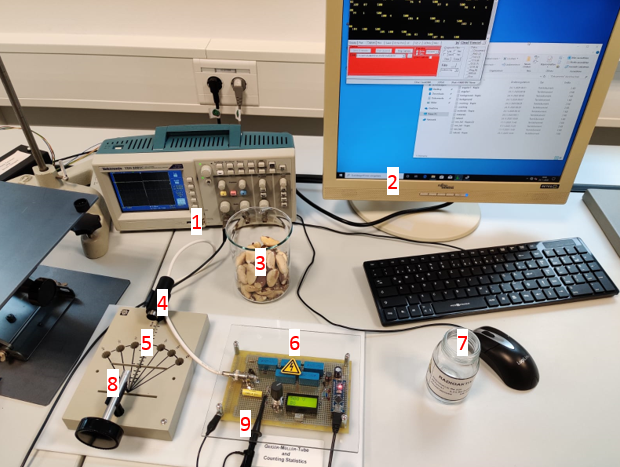
\includegraphics[width=14cm]{setup.png}
		\caption{Equipment and material required for the experiments.}  
		\label{fig:setup} 
	\end{center}
\end{figure}
%
\begin{enumerate}
	\item Oscilloscope
	\item Computer with the software RealTerm
	\item Beaker with Brazil nuts
	\item Geiger-Müller tube
	\item Mounting plate
	\item Circuit board
	\item Protective container
	\item Radioactive source ($^{226}$Ra, 3.3 kBq)
	\item Oscilloscope probe with ground clip
\end{enumerate}
%
A better view of the circuit board will give fig. \ref{fig:circuit_board}. Again, the components are listed below.
%
\begin{figure}[H]
	\begin{center}
		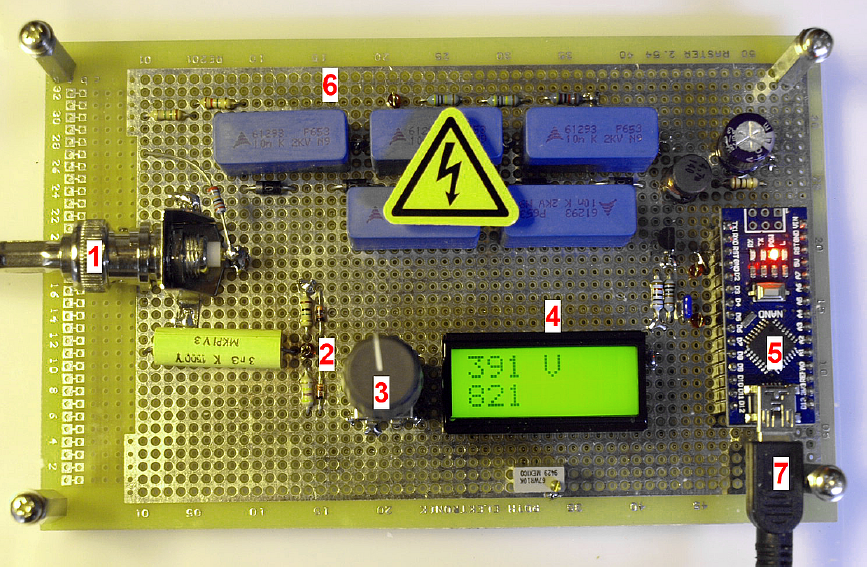
\includegraphics[width=14cm]{circuit_board.png}
		\caption{Circuit board in greater detail. (Source: A. Doerr, Geiger-Mueller Tube and Counting Statistics, page 5)}  
		\label{fig:circuit_board} 
	\end{center}
\end{figure}
%
\begin{enumerate}
	\item BNC connector
	\item Testpoint
	\item Potentiometer
	\item LCD
	\item Arduino nano
	\item Boost converter
	\item USB port
\end{enumerate}
%
To begin with the experiments, the computer is started first. When the computer is ready, the program RealTerm is being started. The following settings are made:
\begin{itemize}
	\item In the \texttt{Port} tab, 9600 is selected for \texttt{Baud}.
	\item The microcontroller is connected with the computer and the assigned COM number is selected under \texttt{Port}.
	\item On the \texttt{Display} tab, \texttt{Ascii} and \texttt{new Line mode} are checked, \texttt{Direct capture} is un-checked.
\end{itemize}
%
The data is now continuously sent by the microcontroller. The data is displayed on the screen. A text file is created in which the data is written and saved. Three columns are displayed. The first column contains the number of the measurement, the second the counts per 10 s and the third the present voltage $U_{GMT}$.\\
Now the oscilloscope is switched on. The probe tip is connected to the test point. The ground clip is attached to the housing of the circuit board. The display is adjusted so that a single radioactive event fills the screen when the trigger is set correctly.\\
Now the setup is completed and the experiments can be started.

\input{chapters/4_durchführung}
\chapter{Evaluation}
\chapter{Conclusion}
%-------------------
\newpage
\listoffigures 
\listoftables
\addchap{Glossary}
\begin{table}[h]
    \begin{tabular}{@{}ll@{}}
        $s$ & Strahlweg\\      
    \end{tabular}
    \label{tab:glossar}
\end{table}
\appendix
\chapter{Appendix}
%\bibliography{Z:/Dokumente/HSRM/LaTex_Quellen/HSRM_Quellen/quellen}
\printbibliography
%\bibliographystyle{plaindin}
%==========================================
\end{document}